% !TeX encoding = utf8
% !TeX spellcheck = pl_PL

\documentclass[11pt, a4paper, twoside]{article}
\usepackage{graphicx, color, rotating} 
\usepackage[MeX, plmath]{polski} %MeX - tryb pełnej polonizacji
\usepackage[OT4]{fontenc} % T1 - skład fontami EC; OT4 - układ fontów PL
\usepackage{ae,aecompl}
\usepackage[utf8]{inputenc}
\usepackage{lmodern} %czcionka latin modern; jednolita dla tekstu i wzorów;
\usepackage{a4wide}
\usepackage{amsmath}
\usepackage{amssymb, latexsym}
\usepackage{array}
\usepackage{bm}
\usepackage[shortlabels]{enumitem}
\usepackage[font=footnotesize]{caption} %rozmiar czcionki podpisów pod rysunkami
\usepackage{float}
\usepackage{subfig} %obrazki obok siebie
\usepackage[hidelinks]{hyperref}
\usepackage{indentfirst}
\usepackage{geometry}
\geometry{left=25mm, right=25mm, top=25mm, bottom=25mm}

\usepackage[final]{pdfpages}
\usepackage{pdflscape}
\prefixing %notacja prefiksowa w pakiecie 'polski'
\frenchspacing
\linespread{1.1}
\renewcommand{\figurename}{Rys.}
\hyphenation{steer-ing}
%\renewcommand*\thesubsection{\arabic{subsection}} % zmiana numeracji podsekcji 0.X -> X

\begin{document}
	
	\begin{center} 
		{\Large Wydział Elektroniki i Technik Informacyjnych}
		\vskip0.2cm
		{\LARGE \textbf{Sieci i sterowanie systemami (SST): Smart City --~raport końcowy po etapie III projektu } } 
		\vskip0.3cm
		{\Large Szymon Jarocki, Daniel Giełdowski, Maciej Kłos, Michał Okoński}
		\vskip0.8cm
	\end{center} 	


\section{Omówienie wyników testów}
\label{sec:Wyniki}
Celem ostatniego etapu była ocena skuteczności działania utworzonego oprogramowania. W~związku z~tym przeprowadziliśmy badania eksperymentalne, których wyniki przedstawiamy w niniejszym rozdziale. Zaprojektowane algorytmy sterowania przetestowaliśmy na 3 przykładowych scenariuszach ruchu uszeregowanych pod kątem stopnia trudności.

%\newpage
\section{Omówienie wyników testów}

Zaprojektowane algorytmy sterowania przetestowano na 3 przykładowych scenariuszach ruchu uszeregowanych pod kątem stopnia trudności.

\subsection{Scenariusz 1 - Wykrywanie kolizji}

W pierwszym scenariuszu zbadano zdolność pojazdów do unikania kolizji. Do wykrywania kolizji pojazdy wykorzystywały czujniki laserowe. Po wykryciu zbliżającej się kolizji, pojazd zatrzymywał się. Po zniknięciu kolizji (np. gdy poprzedzający pojazd ruszył) samochód ruszał ponownie. Przykładowe migawki z symulacji przedstawiono poniżej.

\begin{figure}[!h]
	\centering
	\centering
	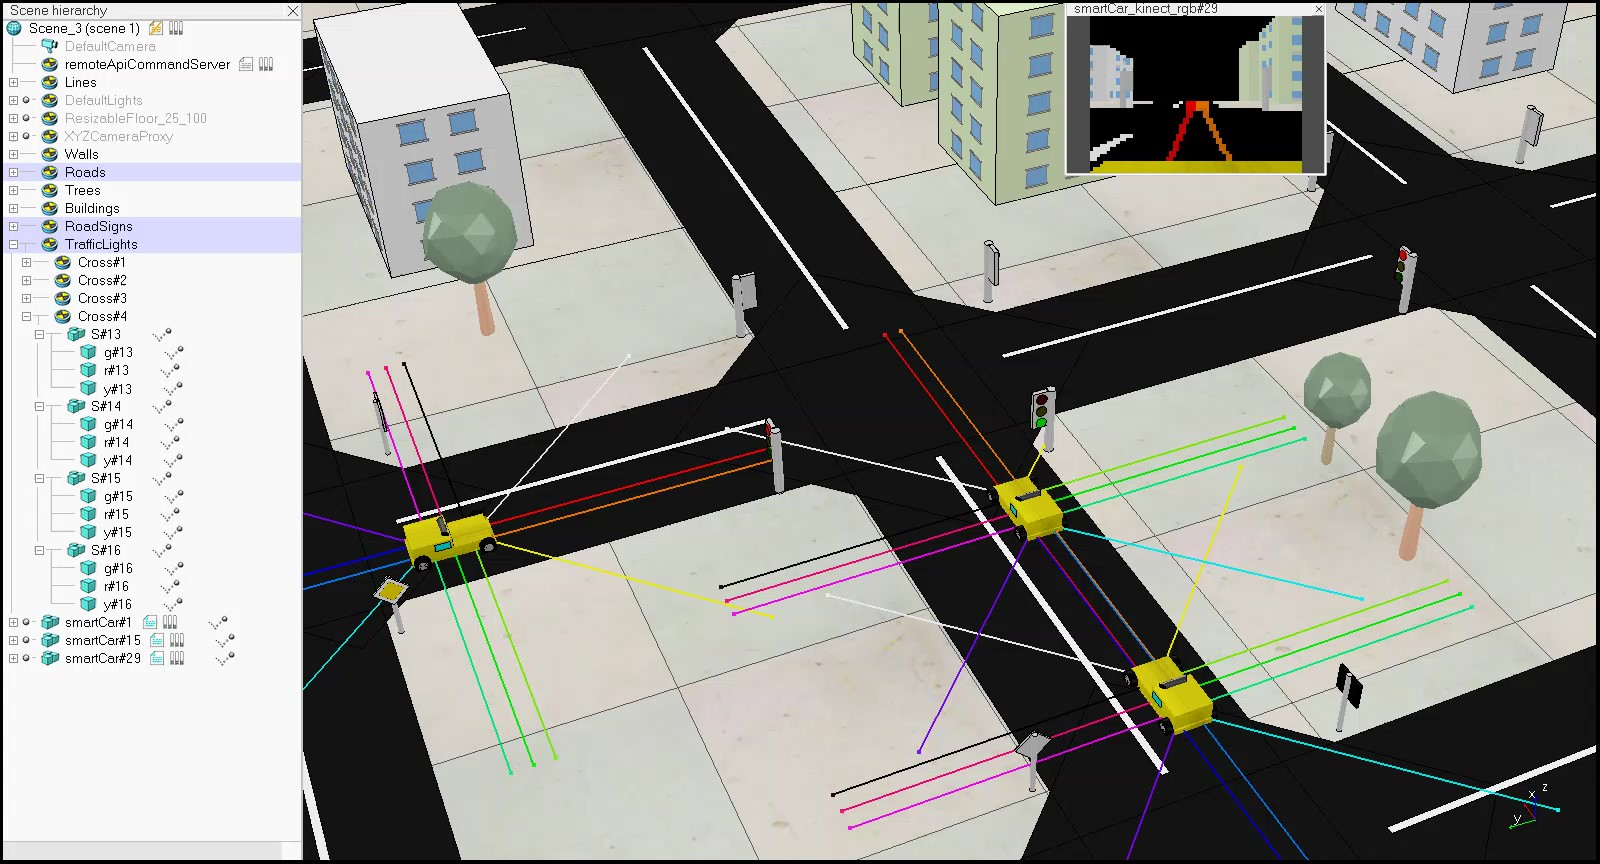
\includegraphics[width=.8\linewidth]{p11.jpg}
	\caption{Początek symulacji - scen. 1}
	\label{fig:p11}
\end{figure}

\begin{figure}[!h]
	\centering
	\centering
	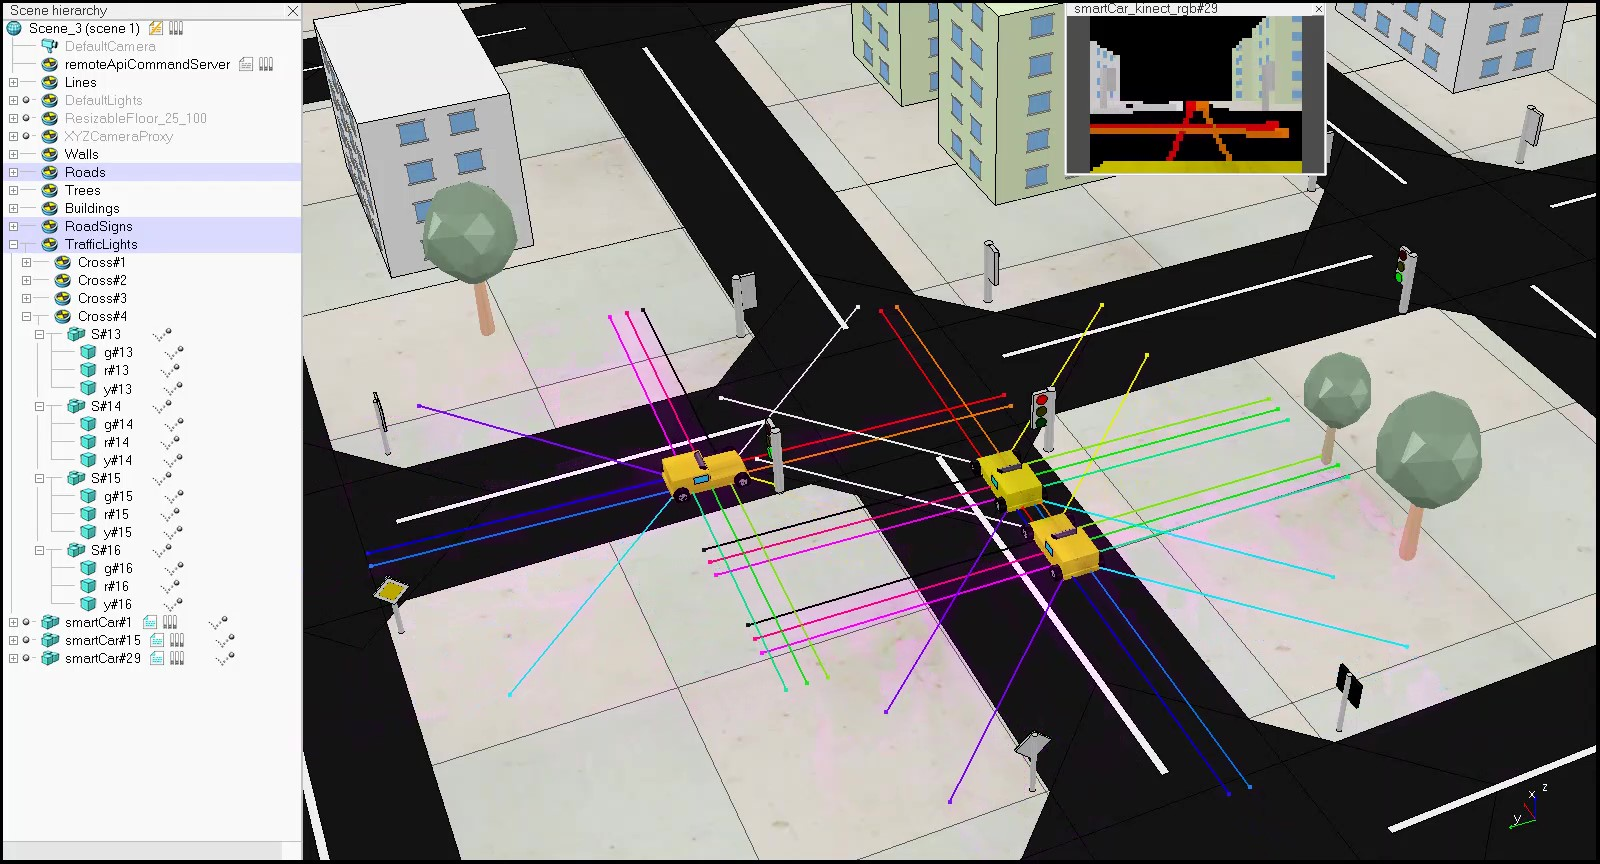
\includegraphics[width=.8\linewidth]{p12.jpg}
	\caption{Wykrycie kolizji po dojeździe do skrzyżowania - scen. 1}
	\label{fig:p12}
\end{figure}

\subsection{Scenariusz 2 - Pokonywanie skrzyżowań}

W drugim scenariuszu zbadano zdolność pojazdów do pokonywania skrzyżowań. Samochody pokonywały skrzyżowania zgodnie z pierwszeństwem wyznaczanym przez zawczasu ustalony priorytet dróg. Samochody zatrzymywały się przed skrzyżowaniem w momencie gdy na drodze o wyższym priorytecie znajdowały się samochody zbliżające się do skrzyżowania. Przykładowe migawki z symulacji przedstawiono poniżej.

\begin{figure}[!h]
	\centering
	\centering
	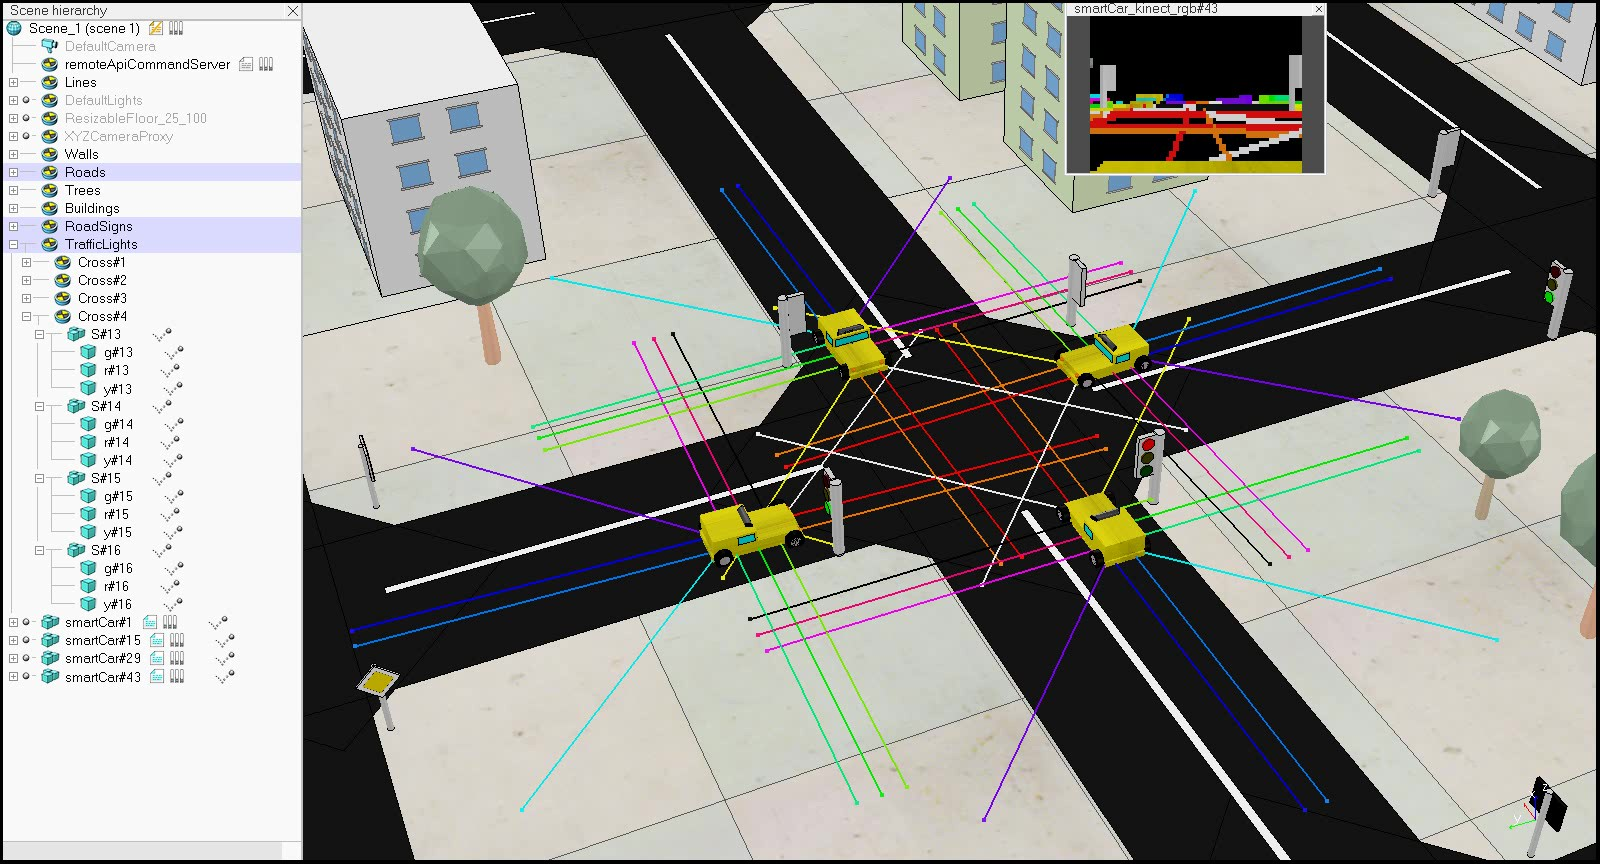
\includegraphics[width=.8\linewidth]{p21.jpg}
	\caption{Początek symulacji - scen. 2}
	\label{fig:p21}
\end{figure}

\begin{figure}[!h]
	\centering
	\centering
	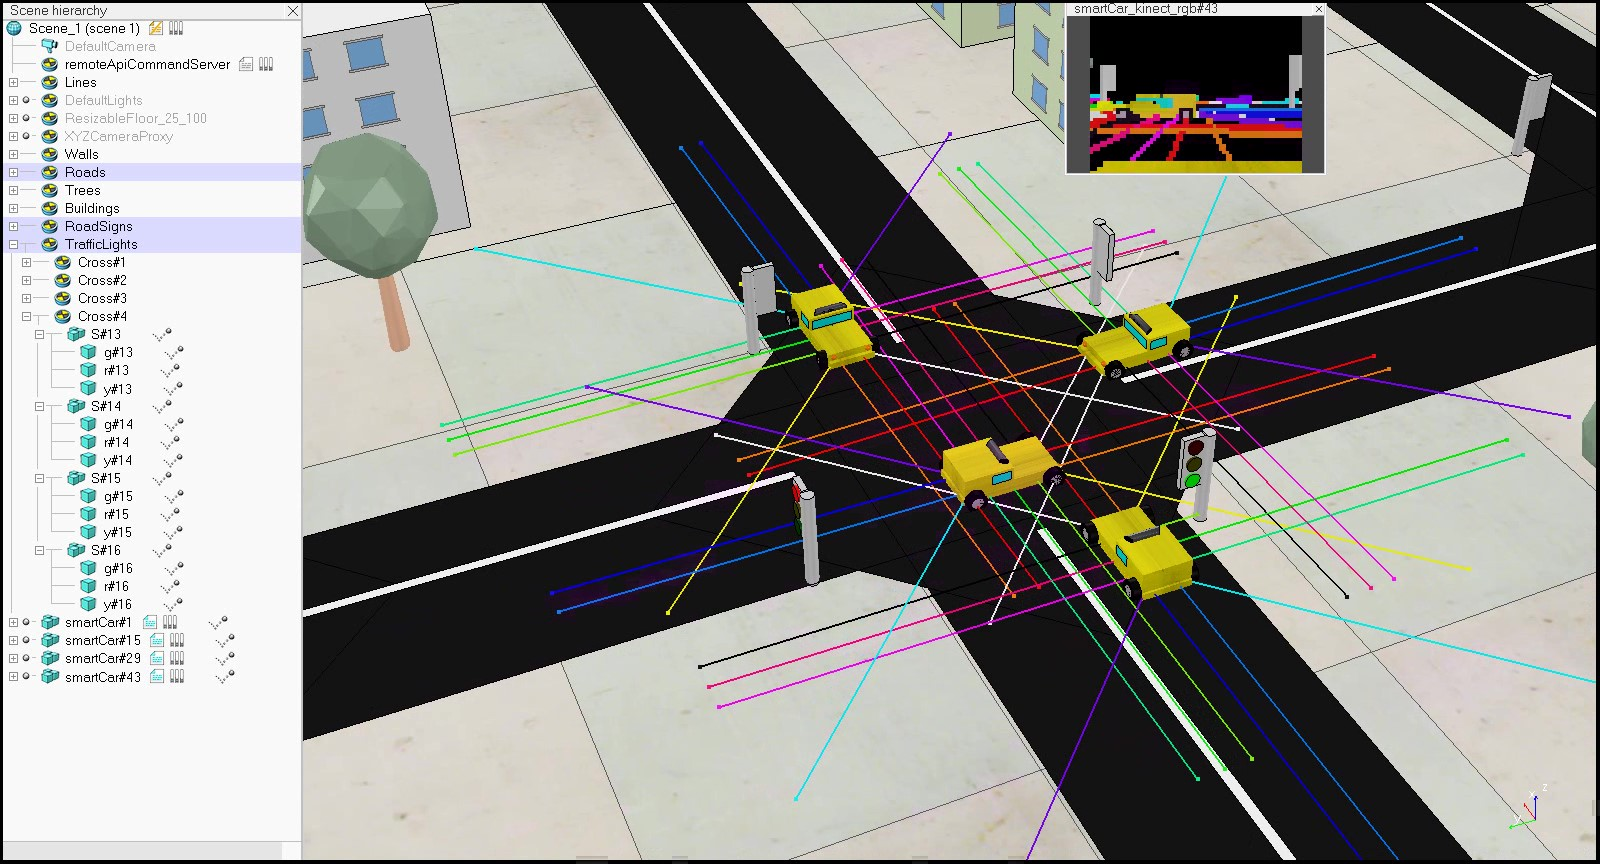
\includegraphics[width=.8\linewidth]{p22.jpg}
	\caption{Przejazd 1. samochodu przez skrzyżowanie - scen. 2}
	\label{fig:p22}
\end{figure}

\begin{figure}[!h]
	\centering
	\centering
	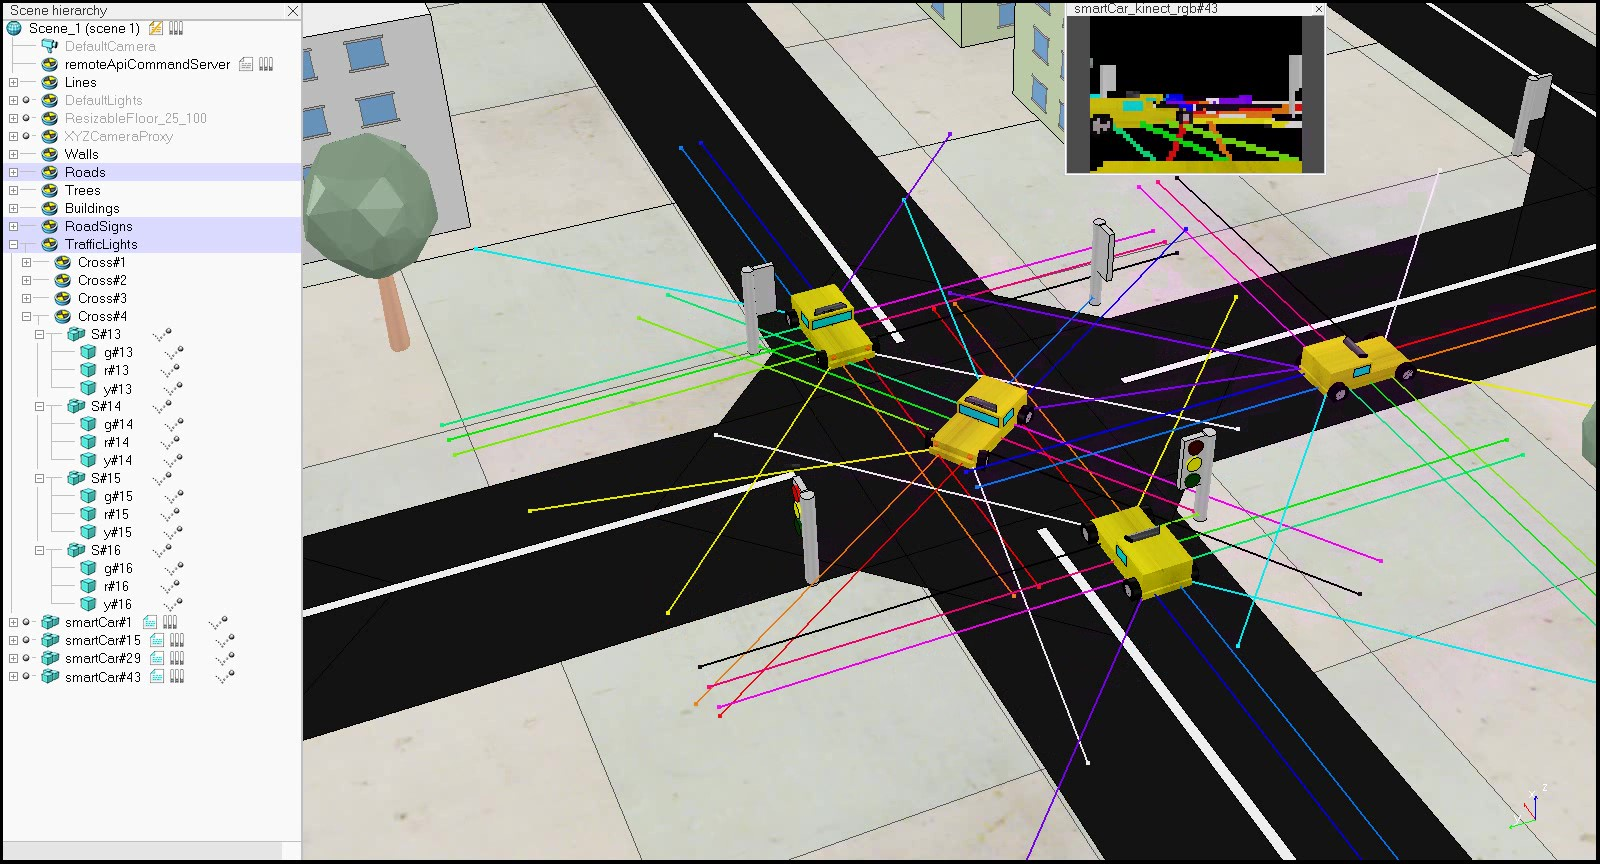
\includegraphics[width=.8\linewidth]{p23.jpg}
	\caption{Skręt w lewo 2. samochodu przez skrzyżowanie - scen. 2}
	\label{fig:p23}
\end{figure}

\begin{figure}[!h]
	\centering
	\centering
	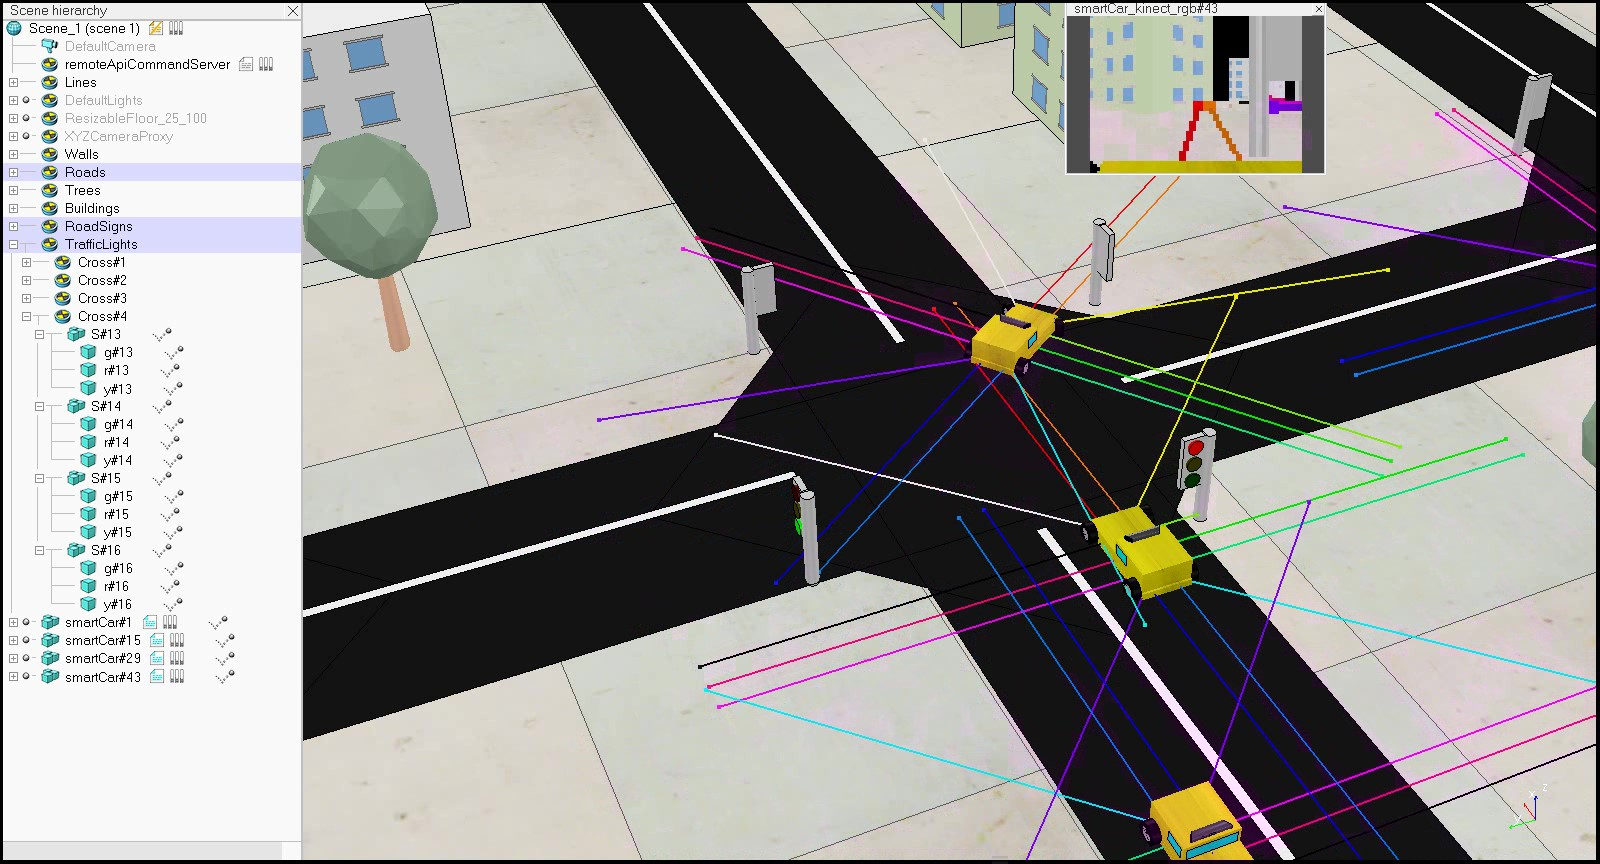
\includegraphics[width=.8\linewidth]{p24.jpg}
	\caption{Zawracanie 3. samochodu na skrzyżowaniu - scen. 2}
	\label{fig:p24}
\end{figure}

\begin{figure}[!h]
	\centering
	\centering
	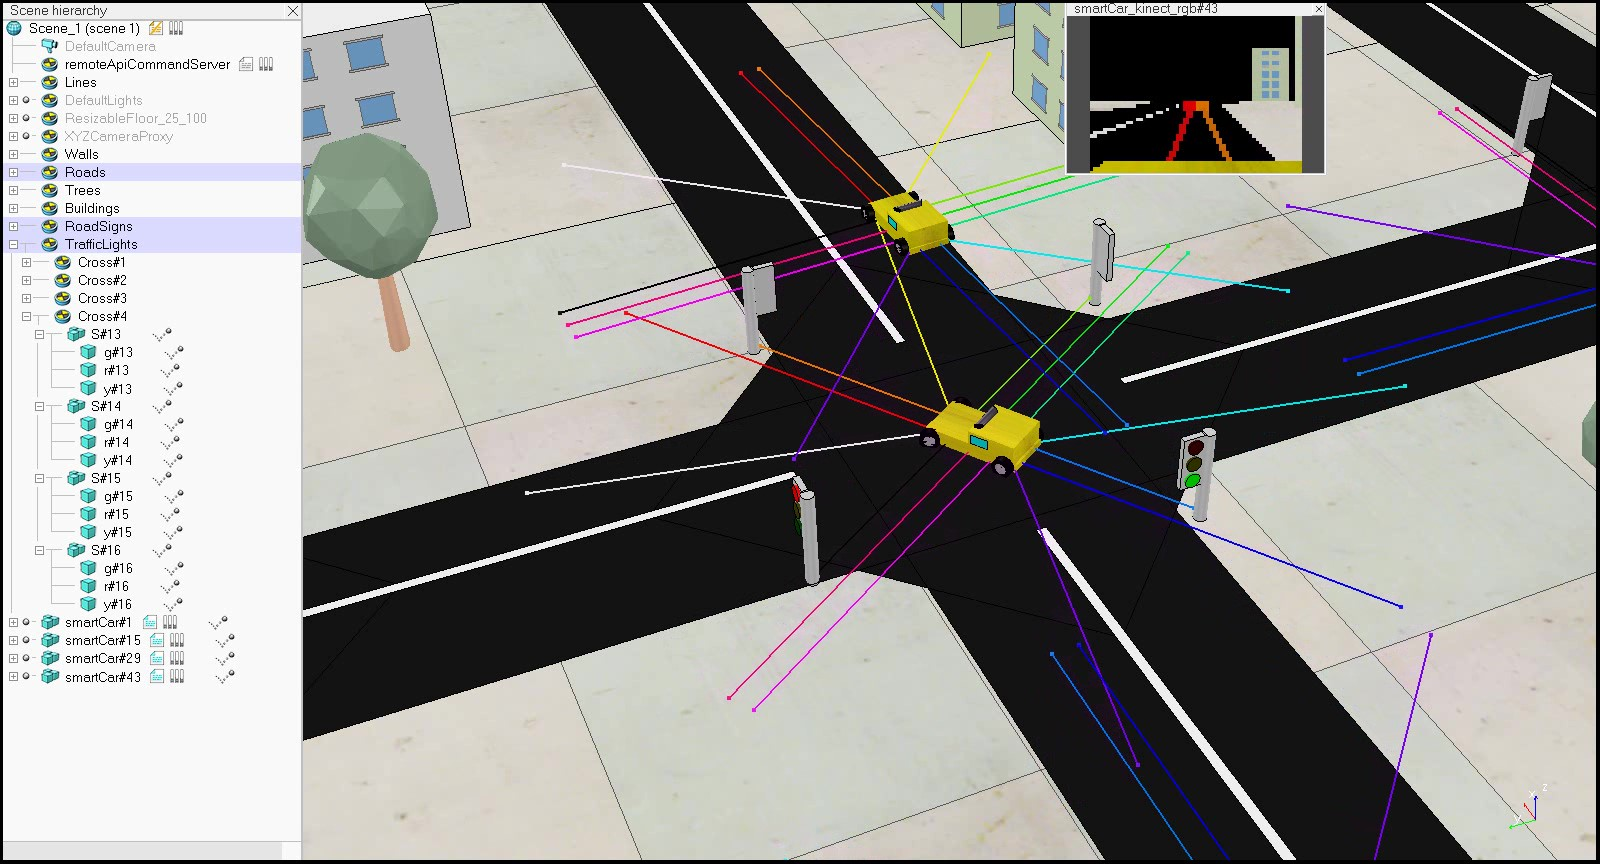
\includegraphics[width=.8\linewidth]{p25.jpg}
	\caption{Zawracanie 4. samochodu na skrzyżowaniu - scen. 2}
	\label{fig:p25}
\end{figure}

\subsection{Scenariusz 3 - Przejazd pojazdów do punktów docelowych}
 
 W ostatnim scenariuszu zbadano zdolność pojazdów do pokonywania zadanych tras w obliczu dużego ruchu. Przeprowadzono symulację z 8 samochodami, którym punkty docelowe zadano w sposób losowy. Przykładowe migawki z symulacji przedstawiono poniżej.
 
 \begin{figure}[!h]
 	\centering
 	\centering
 	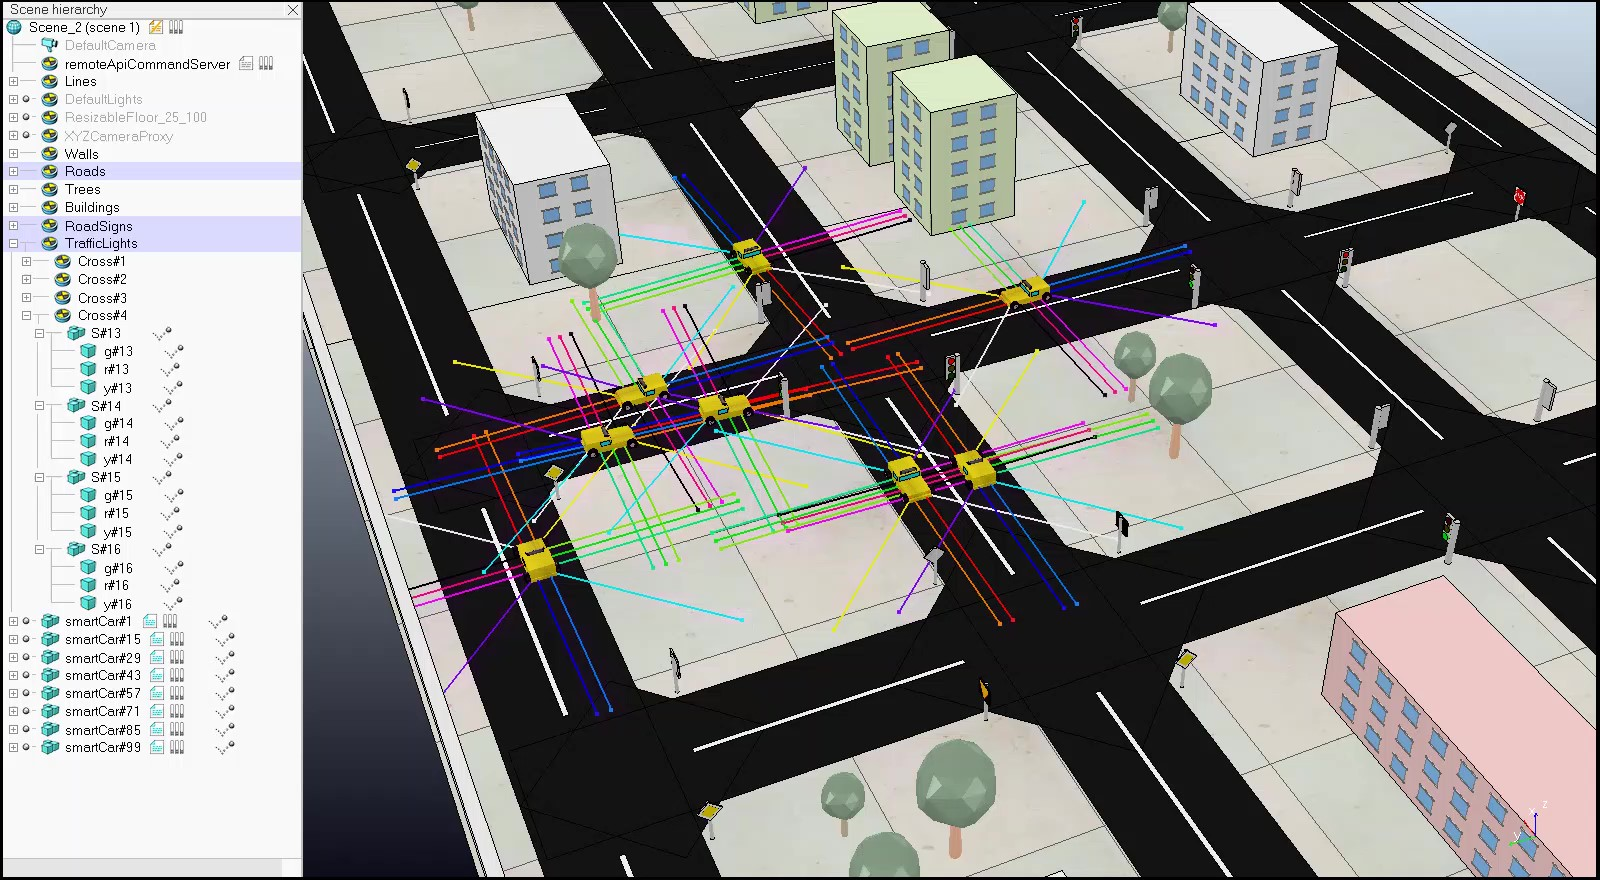
\includegraphics[width=.8\linewidth]{p31.jpg}
 	\caption{Początek symulacji - scen. 3}
 	\label{fig:p31}
 \end{figure}

 \begin{figure}[!h]
	\centering
	\centering
	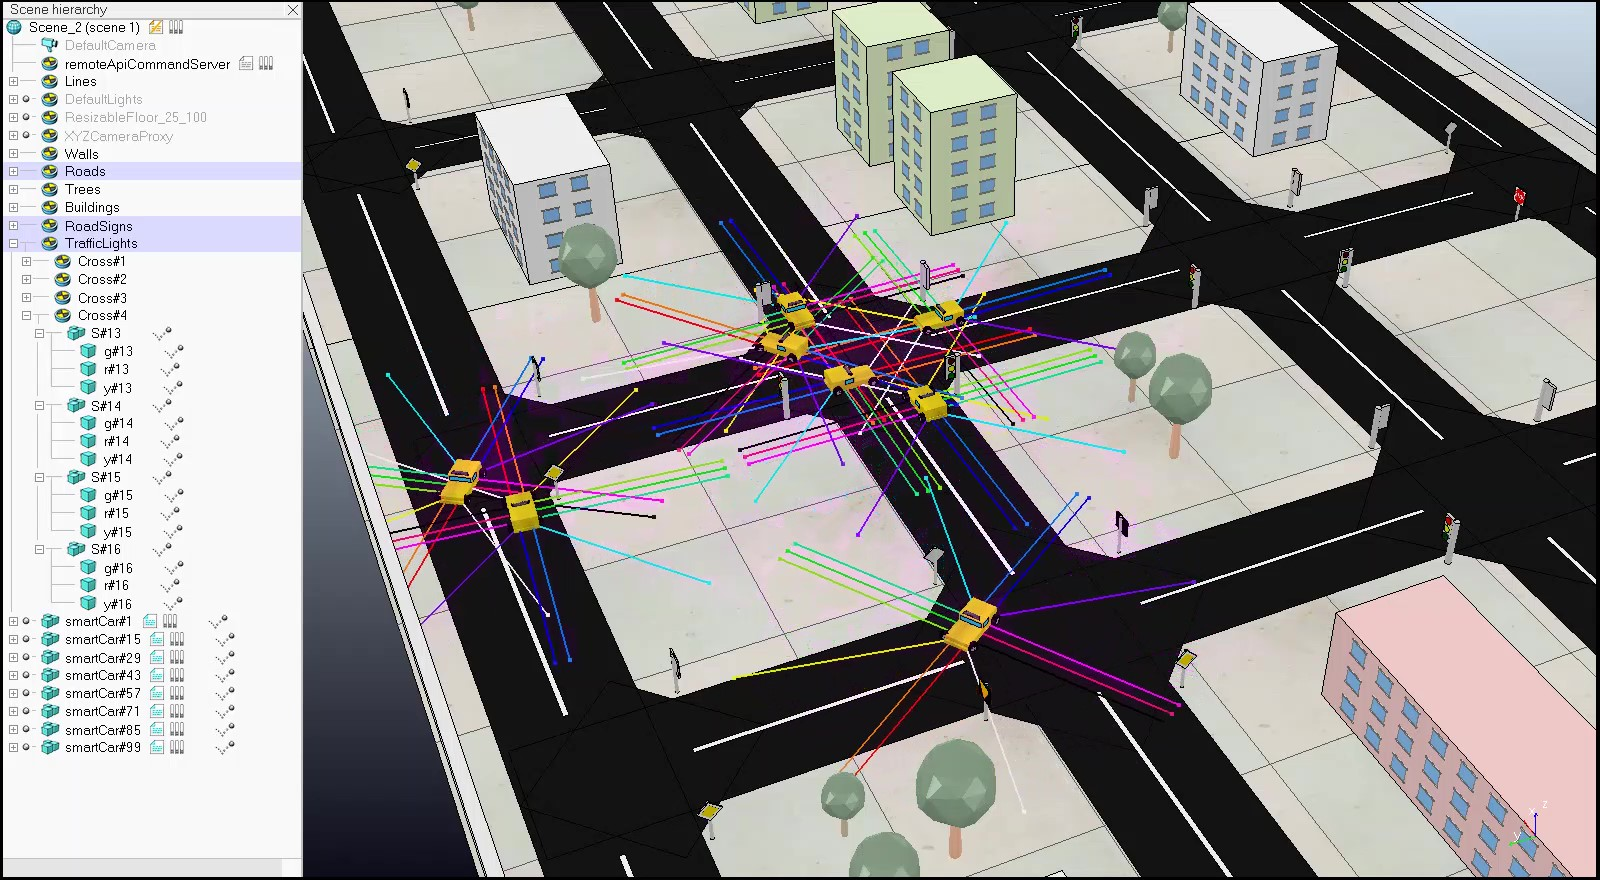
\includegraphics[width=.8\linewidth]{p32.jpg}
	\caption{Migawka z symulacji - scen. 3}
	\label{fig:p32}
\end{figure}

 \begin{figure}[!h]
	\centering
	\centering
	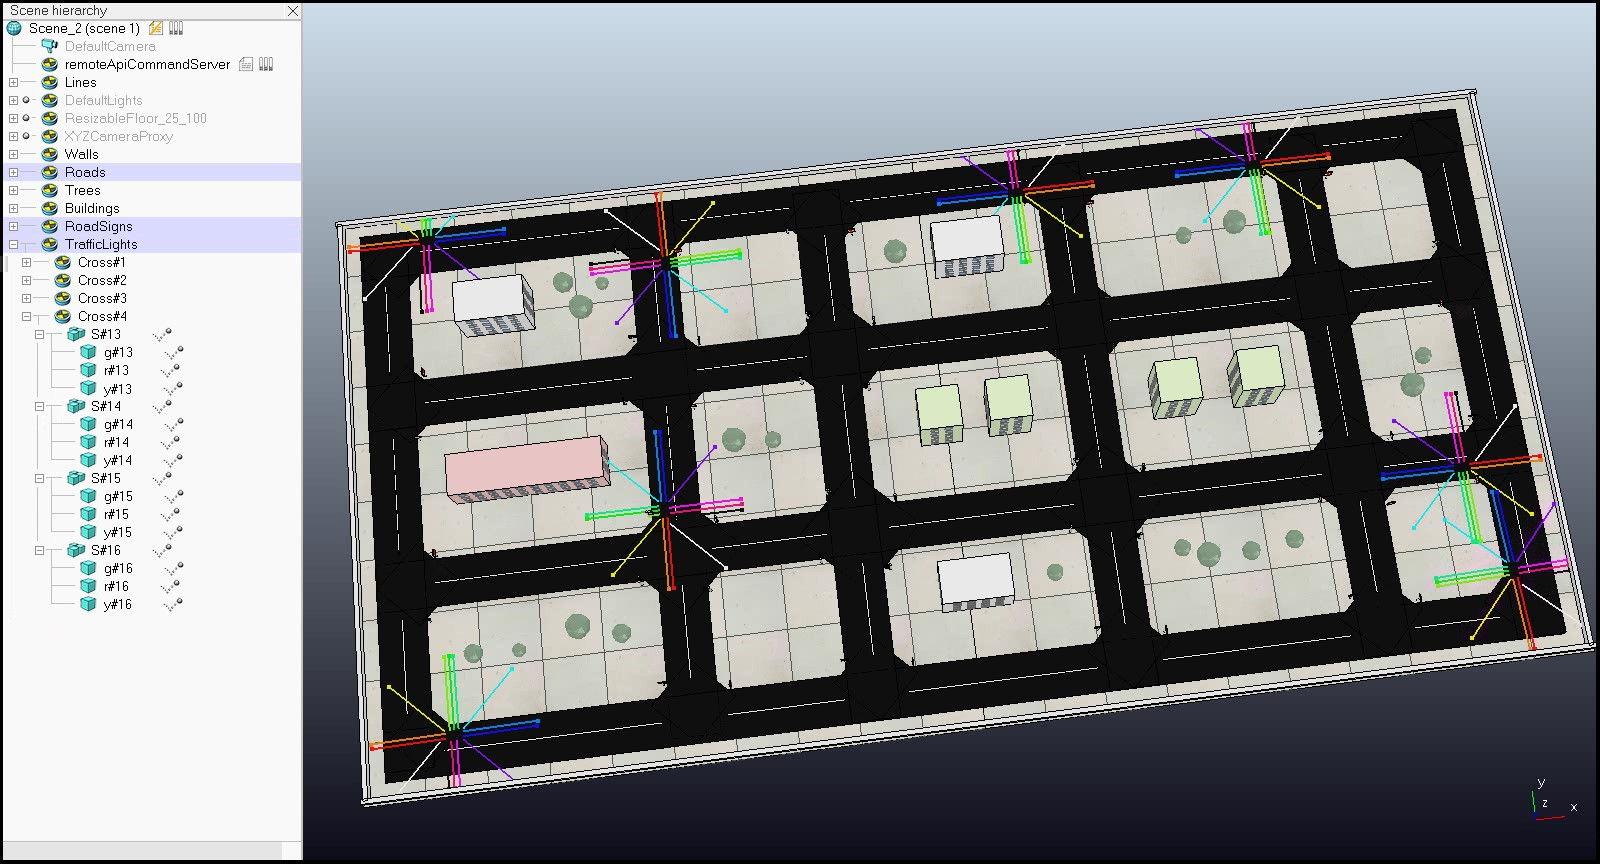
\includegraphics[width=.8\linewidth]{p33.jpg}
	\caption{Koniec symulacji - zaznaczone końcowe pozycje - scen. 3}
	\label{fig:p33}
\end{figure}
 
 
 



\section{Podsumowanie, ocena pracy z symulatorem i perspektywy dalszych prac}
\label{sec:Final}
Zadania i cele projektu zostały zrealizowane, gdyż jako efekt końcowy zaimplementowano symulator grupy autonomicznych samochodów, które poruszają się w~obrębie stworzonego modelu dzielnicy miasta. Pojazdy zostały specjalnie zaprojektowane na~potrzeby projektu i~wyposażone w~odpowiednie czujniki. Strategia sterowania jest realizowana w~programie MATLAB, docelowy symulator w~systemie \mbox{V-REP}, a~wszystko to możliwe jest dzięki odpowiedniej komunikacji pomiędzy tymi programami. Do~zalet symulatora należy przede wszystkim jego intuicyjna wizualizacja, która sprawia, że symulacje mogą zostać zaprezentowane szerokiemu gronu odbiorców, a~ich ogląd nie wymaga specjalistycznej wiedzy. Ponadto zastosowane zostało sterowanie autonomiczne oraz w~uproszczeniu zachowano zasady ruchu drogowego według polskiego prawa.

Pracę z~symulatorem (program V-REP) możemy uznać za~dość sprawną ze~względu na~aspekty obliczeń fizycznych. Odwzorowane są one dobrze i~jednocześnie czas trwania symulacji był w~naszych warunkach (prosty model pojazdu) zbliżony do~rzeczywistego, co~jest niewątpliwą zaletą w~porównaniu z~innymi znanymi nam symulatorami (np. Gazebo). Z~drugiej strony przygotowanie modelu dzielnicy jest żmudne, a~ponadto brakuje takiej funkcjonalności, jak edycja kształtu obiektu. Co~więcej, nie ma niektórych podstawowych kształtów (np. trójkąta), nie mówiąc już o~pewnych bardziej złożonych funkcjach. Niemniej jednak istnieje sporo gotowych obiektów, które można zaadaptować na~potrzeby tworzonych modeli. 

Stworzony symulator możemy potraktować jako produkt w~wersji bazowej, ponieważ zasadniczo algorytm sterowania działa, jednak możliwe jest dodanie nowych funkcjonalności czy też ulepszenie istniejących. W~szczególności warto byłoby rozważyć więcej rodzajów skrzyżowań i~lepiej odwzorować rzeczywiste sytuacje na~drogach. Ponadto sam pojazd może być rozwijany, chociażby poprzez dodanie różnego rodzaju czujników oraz wierniejsze (bliższe rzeczywistości) eksploatowanie istniejących. Wreszcie można by zastosować bardziej zaawansowane strategie sterowania. Na~przykład zamiast najprostszego wariantu z~wagami krawędzi w~grafie równymi długości dróg, warto zastosować choćby wariant z~wartościami wag odpowiadającymi minimalnemu czasowi przejazdu przy uwzględnieniu obserwacji otoczenia. 
		
		
\end{document}

